\section{Schematics} \label{sec:appendix:schematics}

This appendix contains the full hardware schematics for the Synapse-191 computer. Each schematic corresponds to a specific module described in Section \ref{sec:implementation} of this report, including the Control Unit, Register Driver, IO Module, and various registers and memory components.

The schematics have been included  pages for clarity and resolution. They provide a detailed view of the wiring, chip connections, and signal routing used in the physical implementation, but often do not include things like denoising capacitors or LED indicators. The diagrams are intended to complement the modular descriptions in the main text and serve as a reference for replication, debugging, or further development.

All schematics were created during the final build phase and reflect the working configuration of the system as tested.

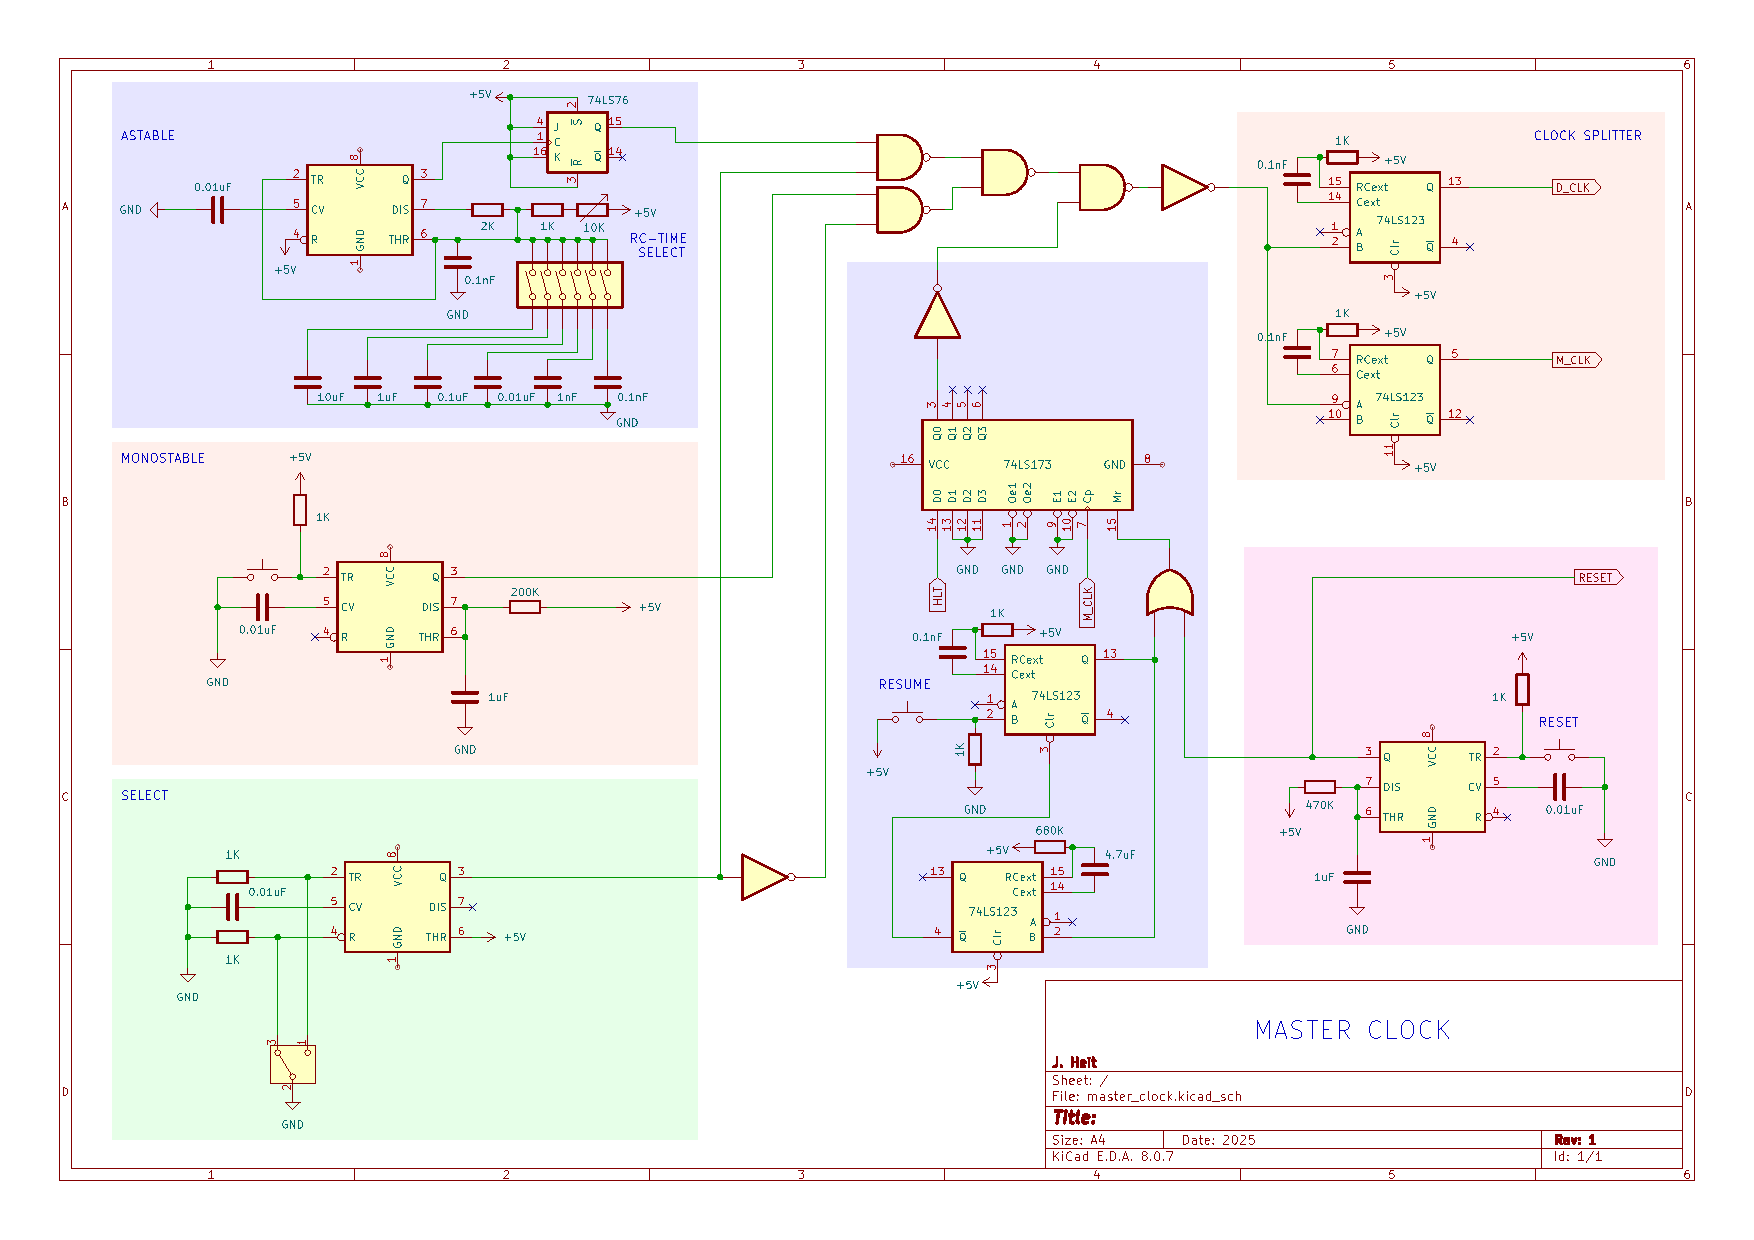
\includepdf[landscape=true]{schematics/masterclock.pdf}
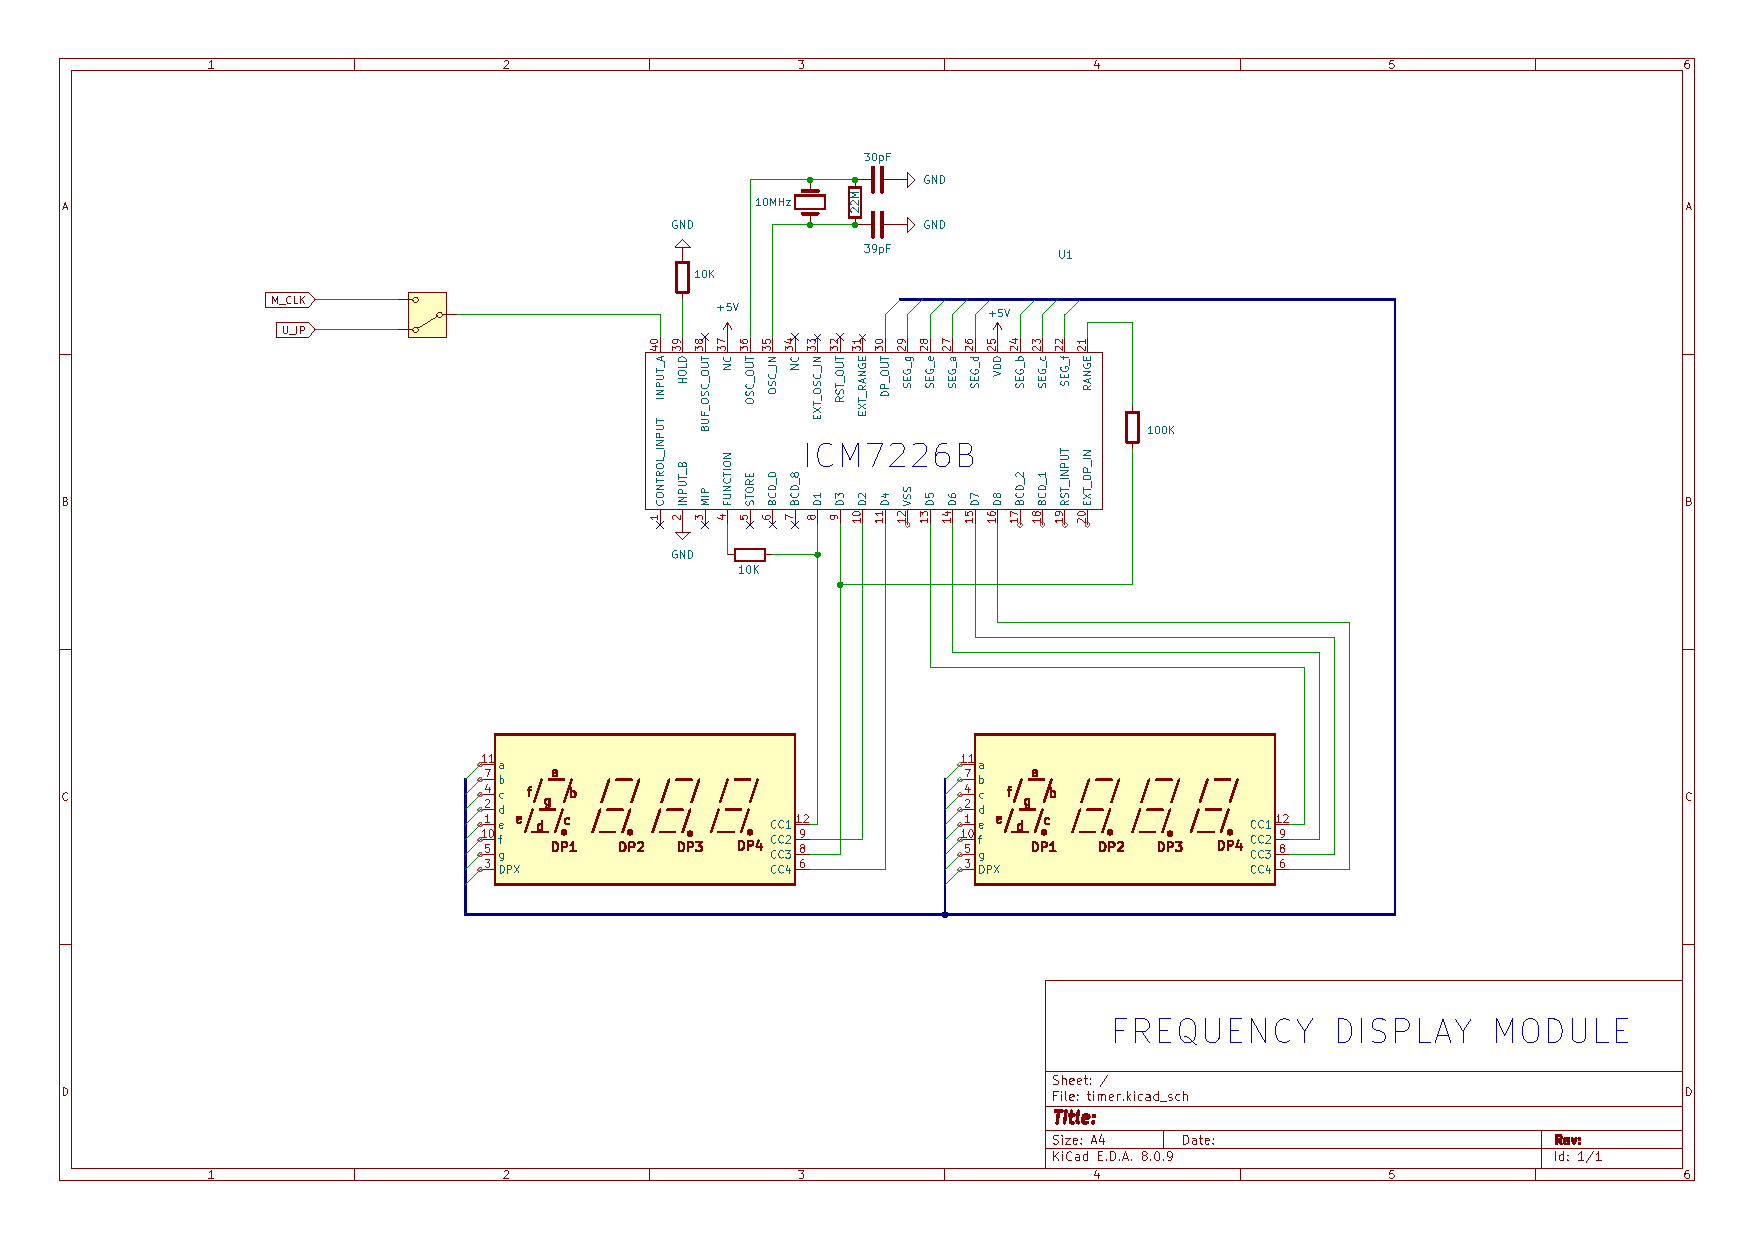
\includepdf[landscape=true]{schematics/frequencydisplay.pdf}
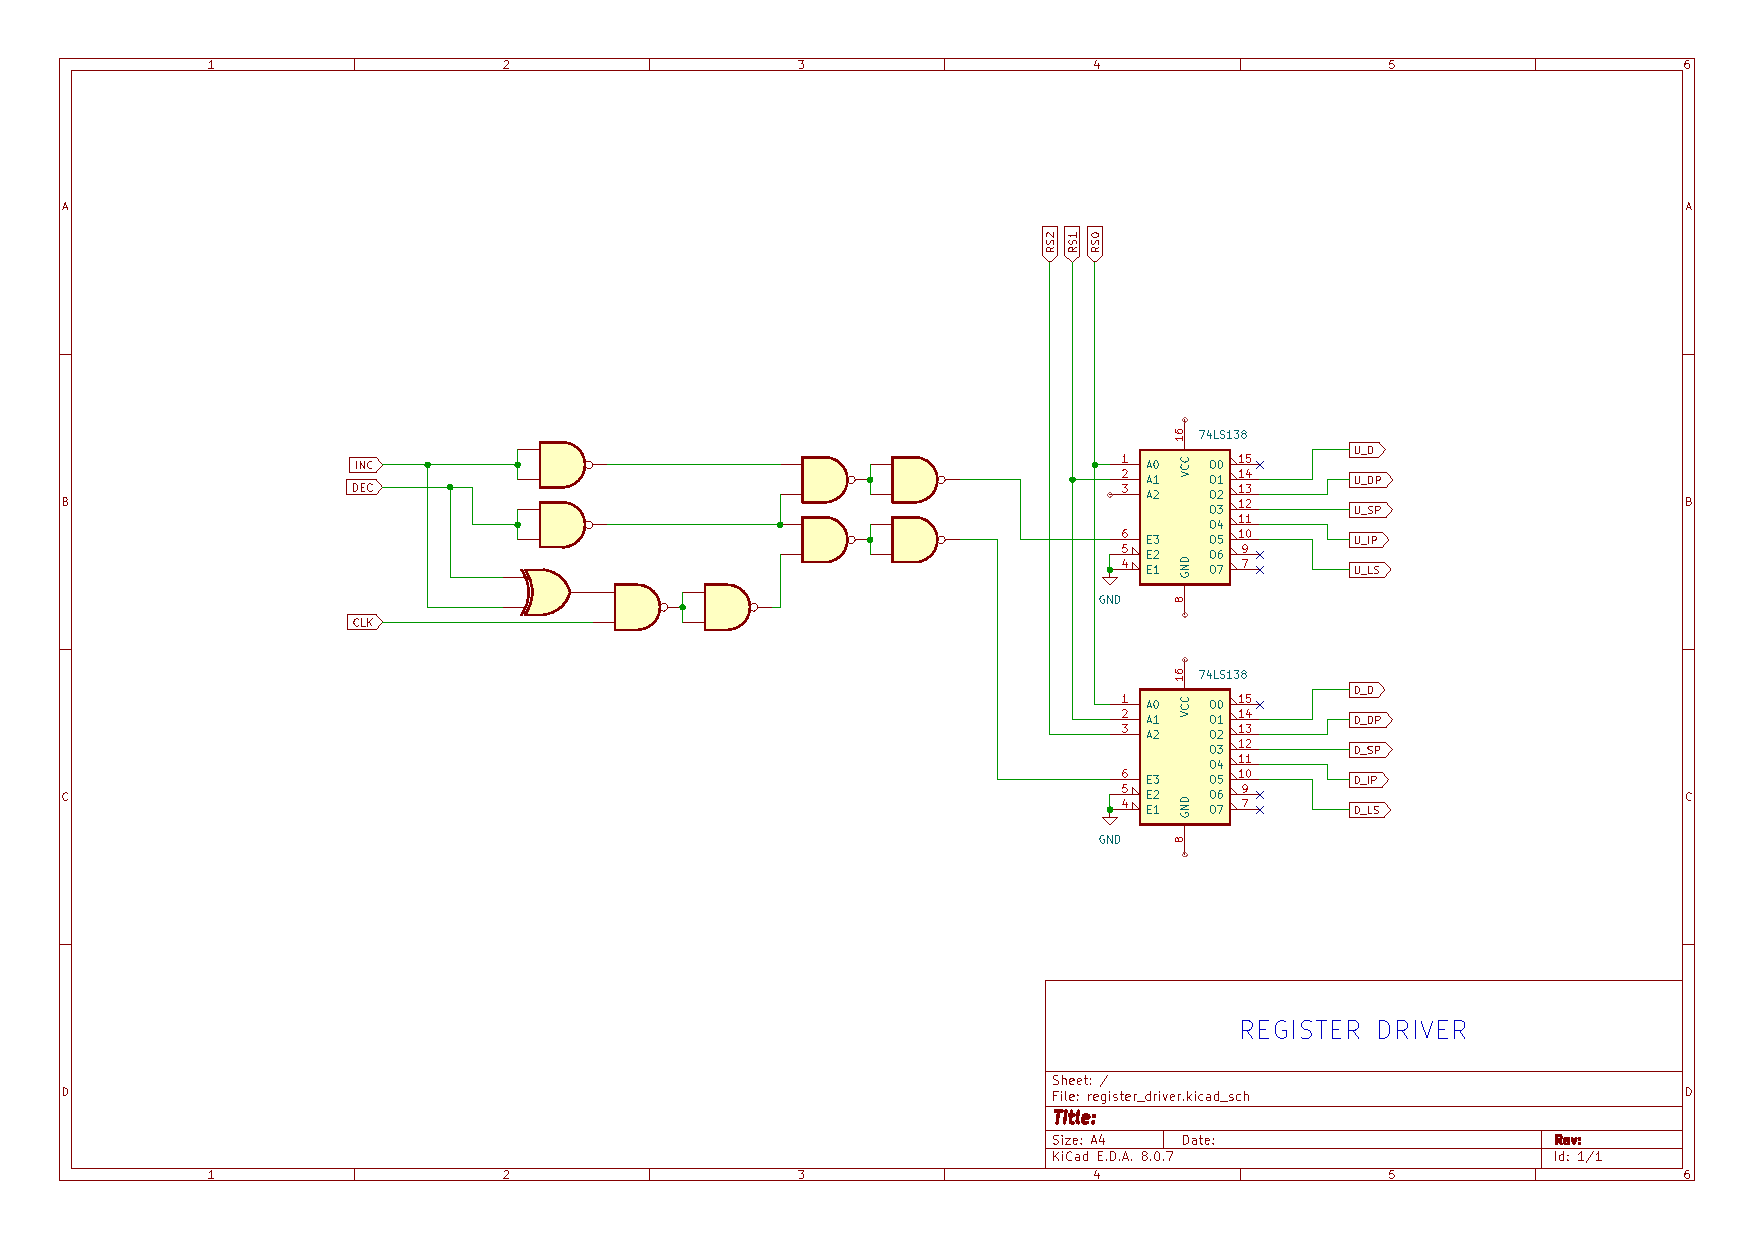
\includepdf[landscape=true]{schematics/registerdriver.pdf}
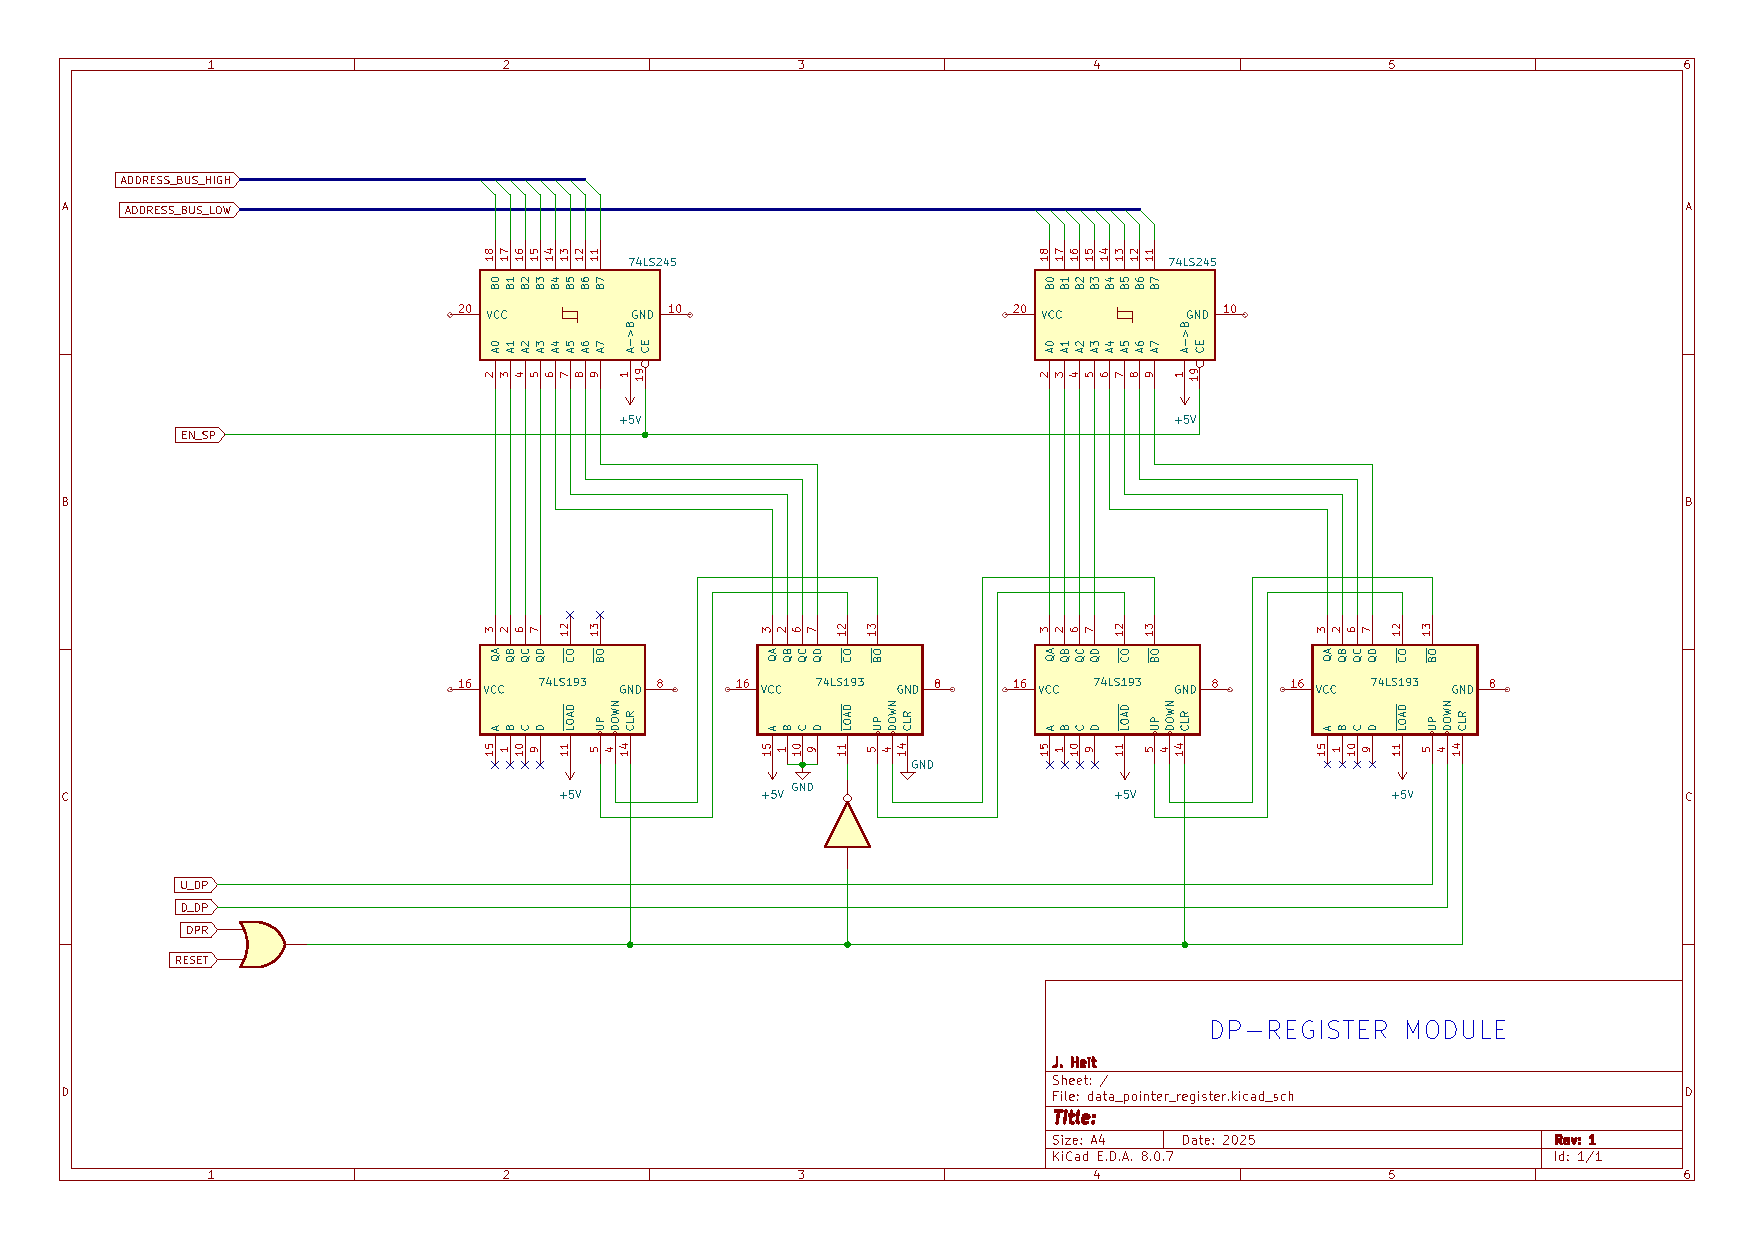
\includepdf[landscape=true]{schematics/datapointerregister.pdf}
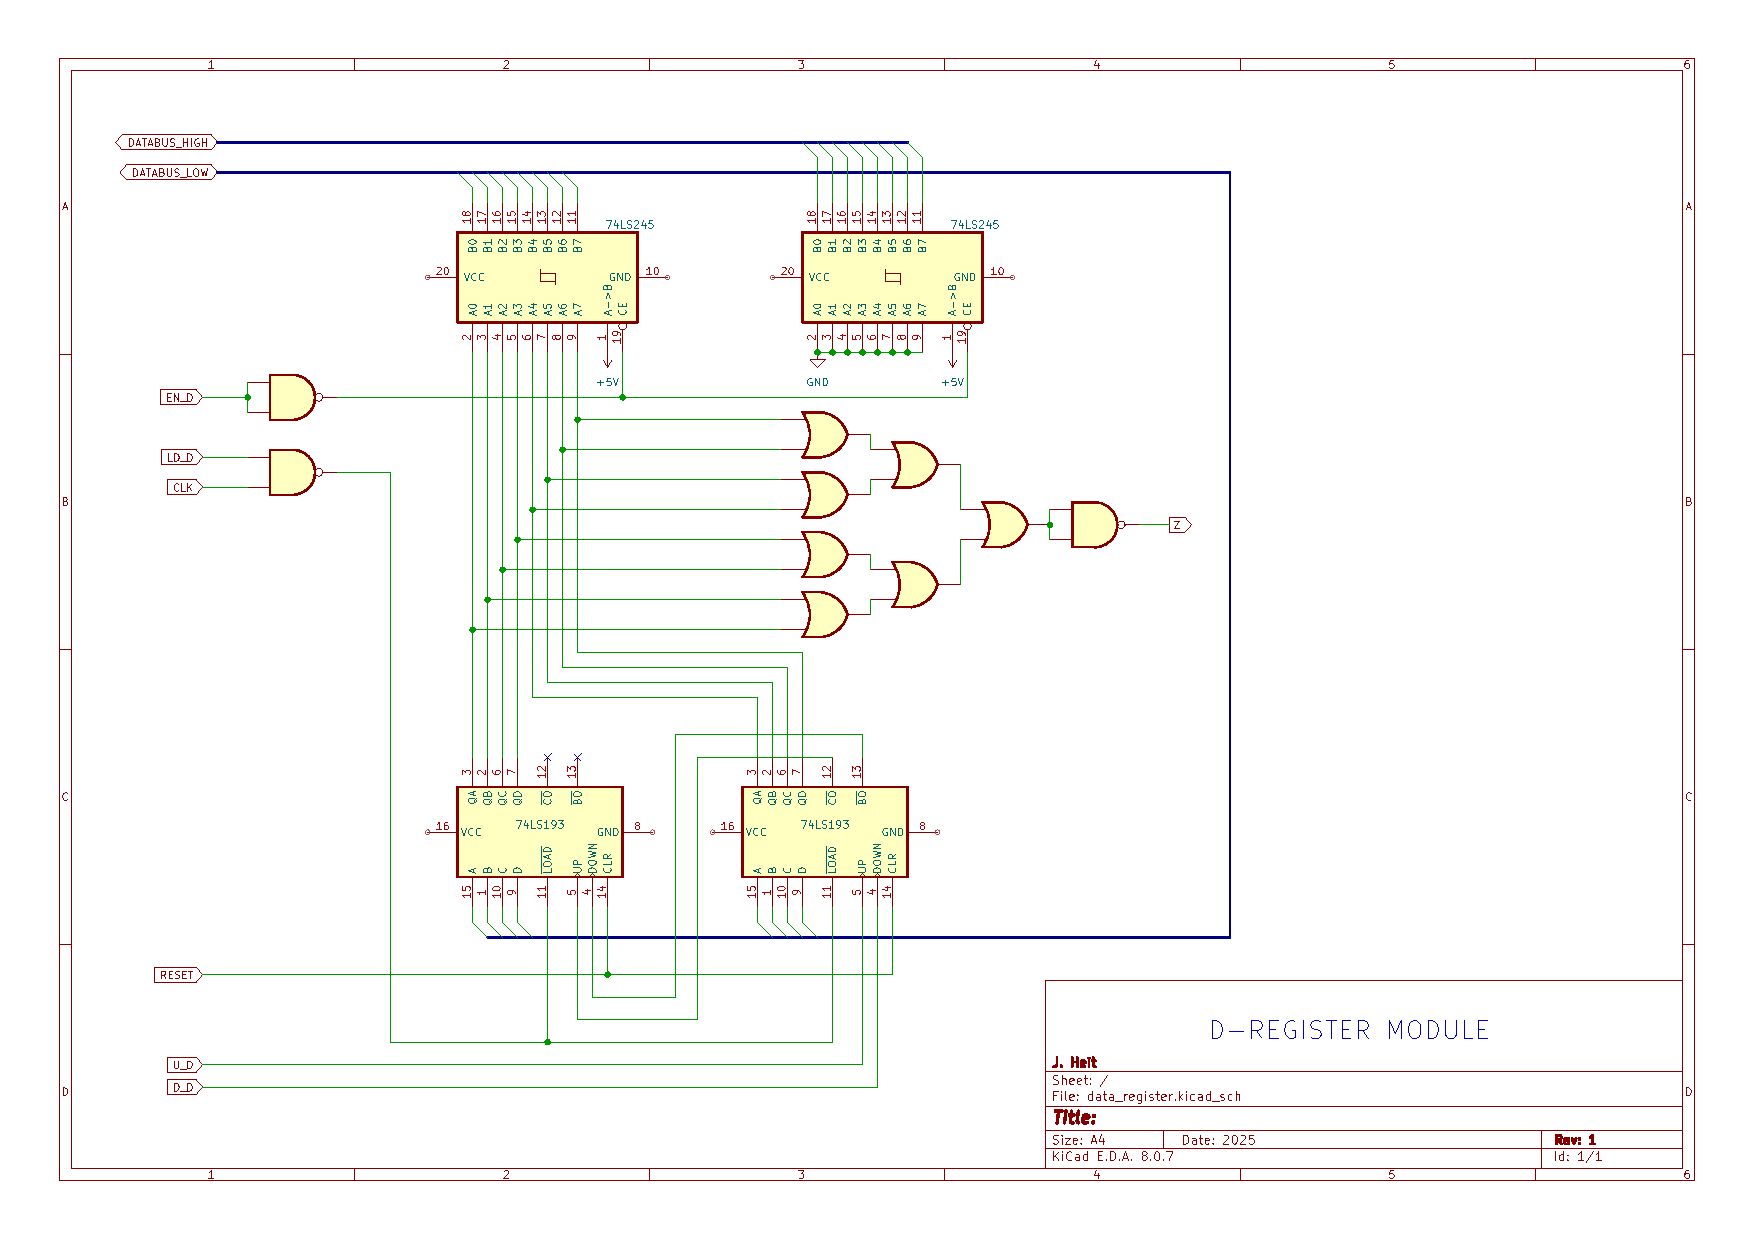
\includepdf[landscape=true]{schematics/dataregister.pdf}
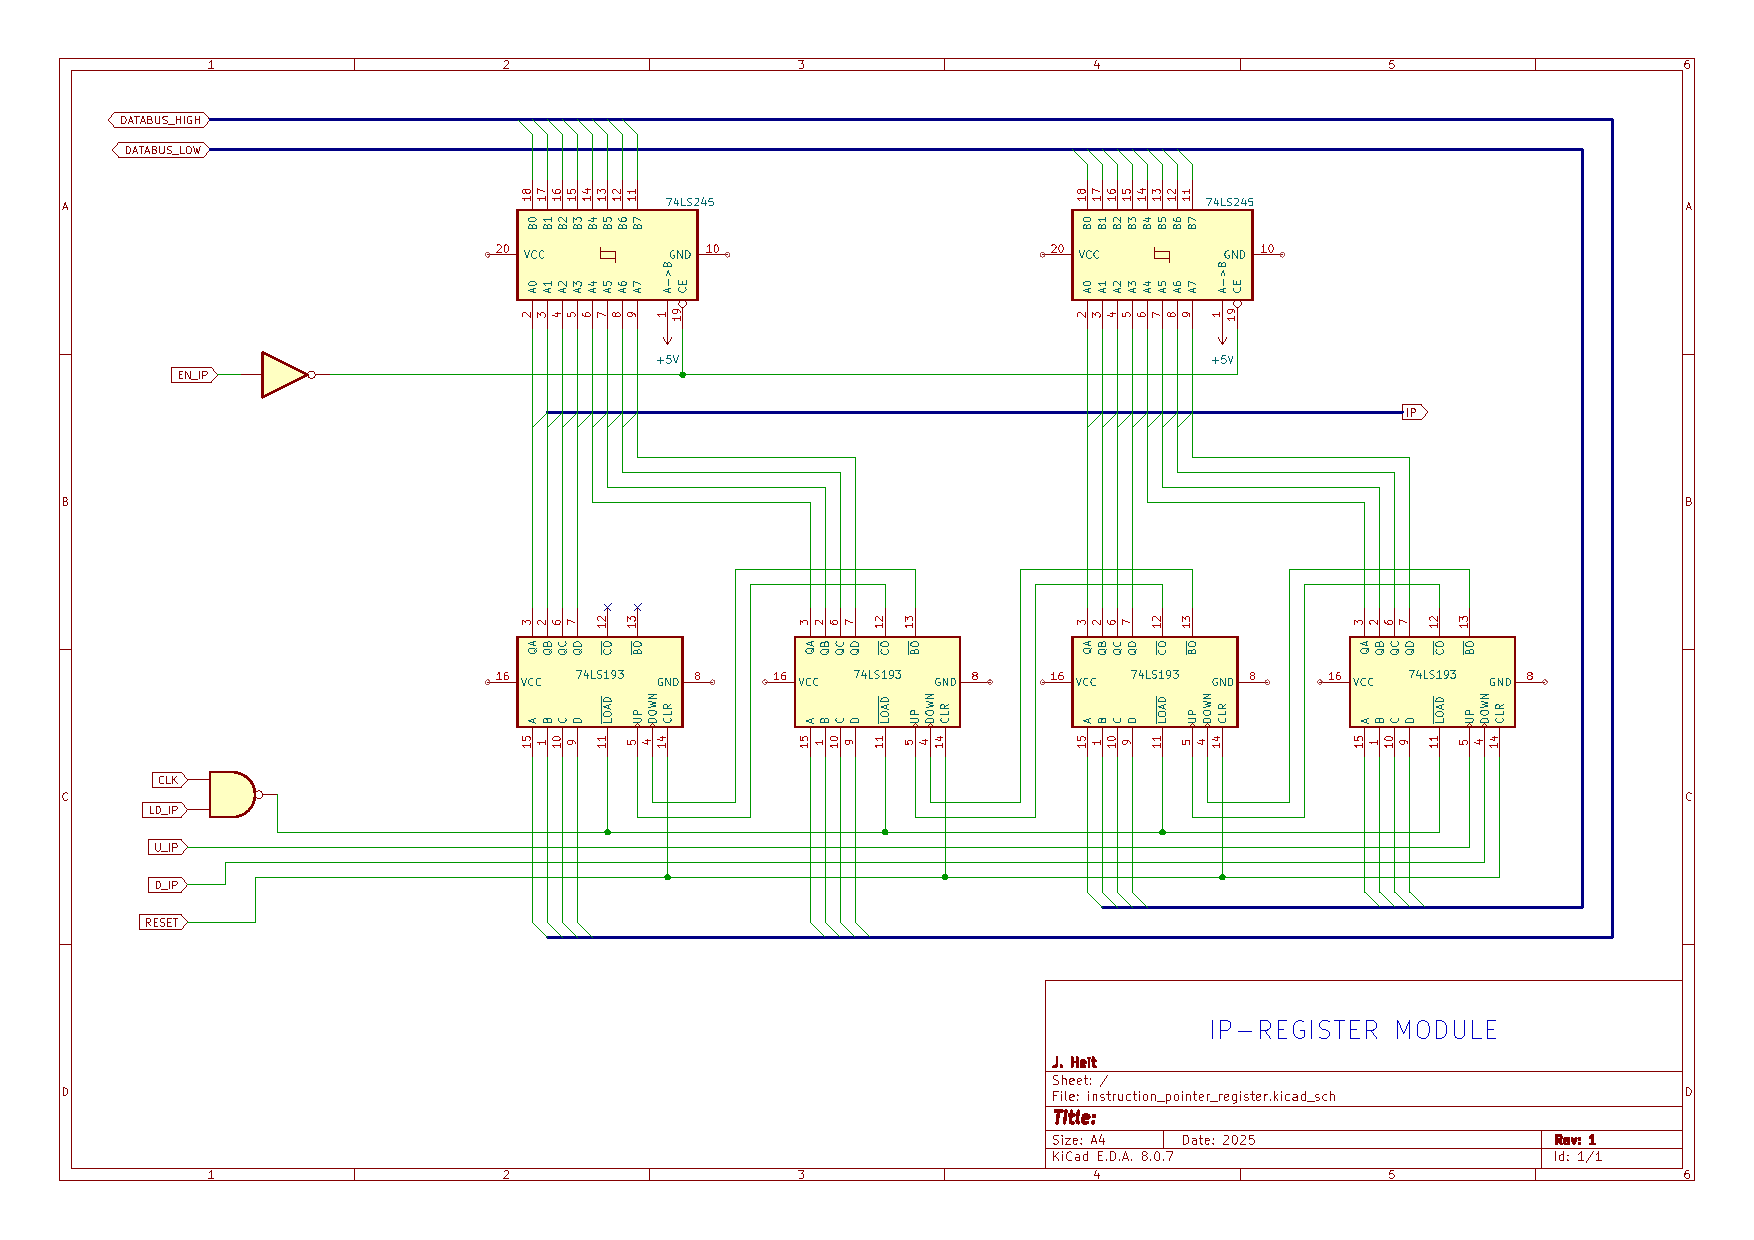
\includepdf[landscape=true]{schematics/instructionpointerregister.pdf}
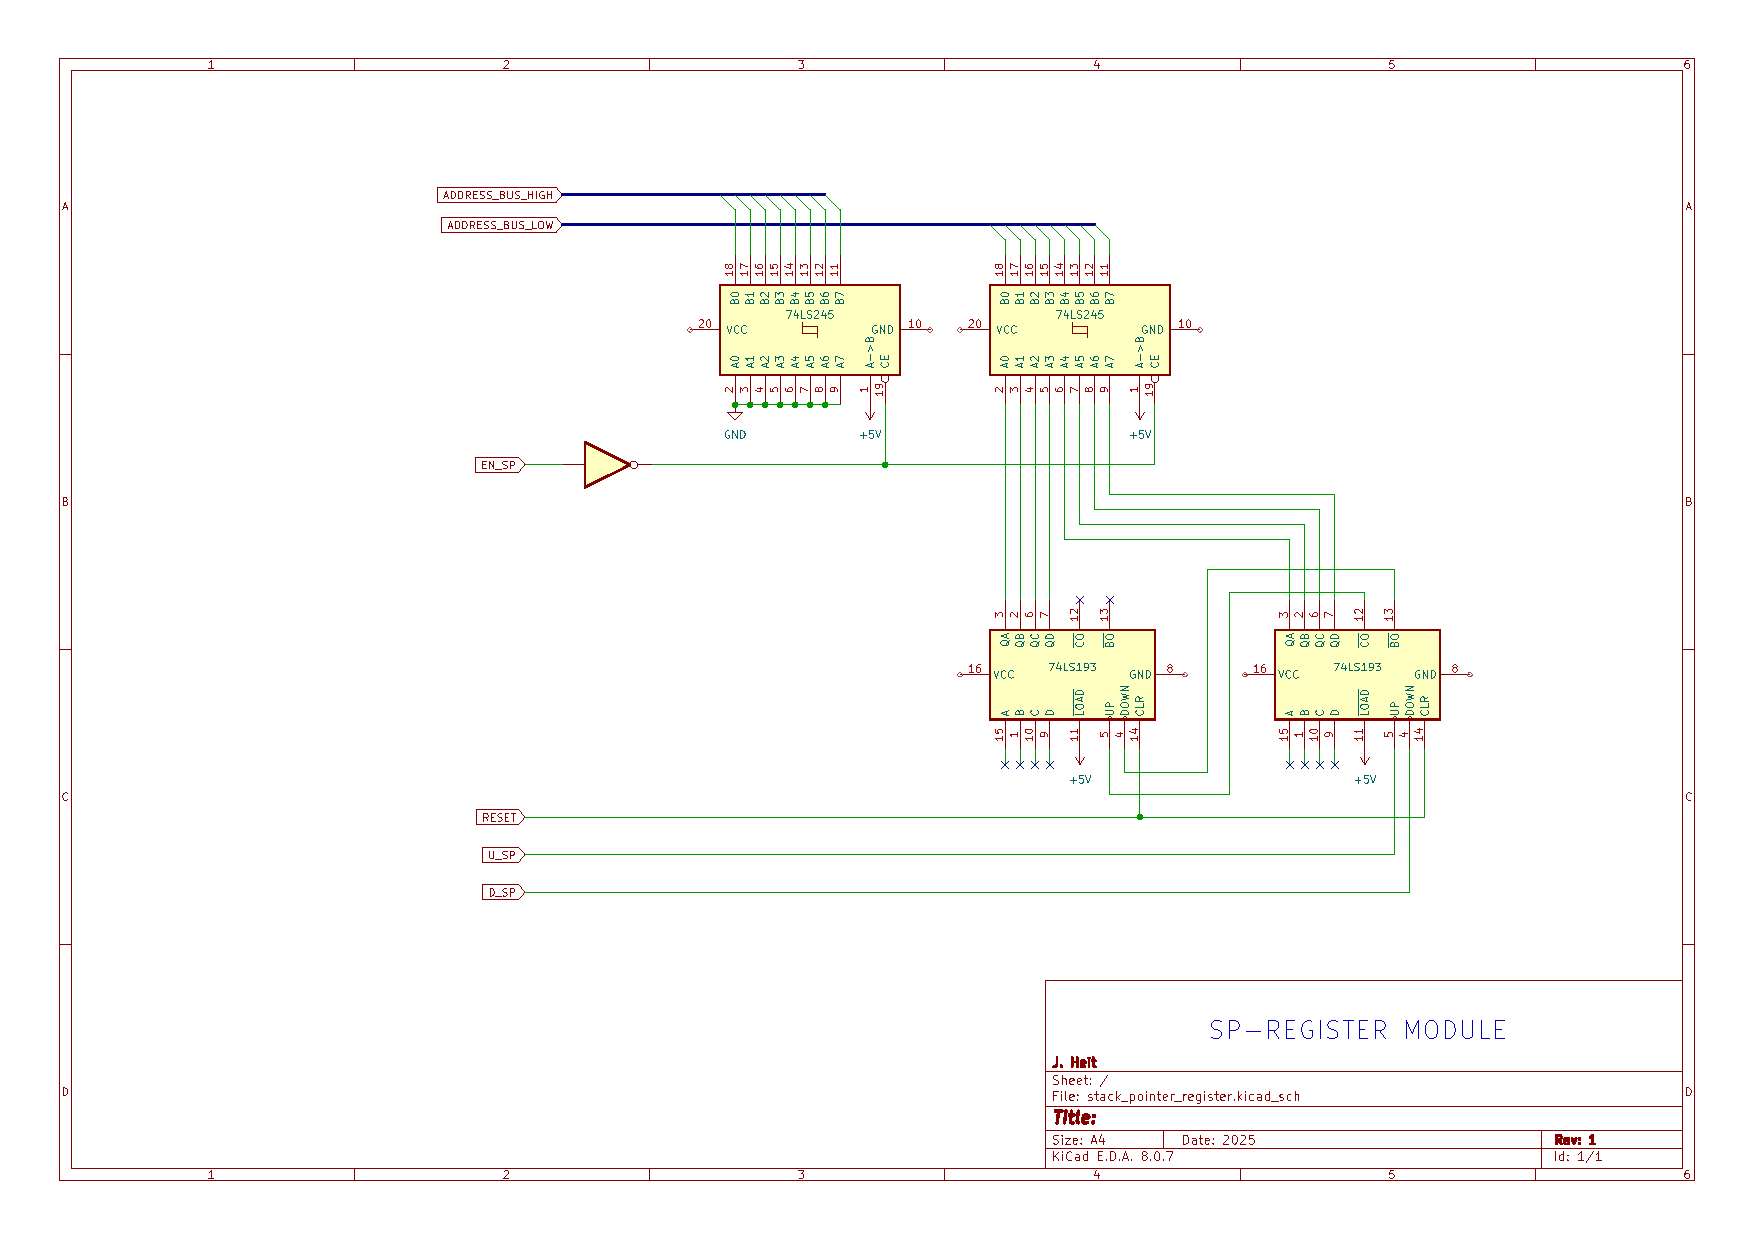
\includepdf[landscape=true]{schematics/stackpointerregister.pdf}
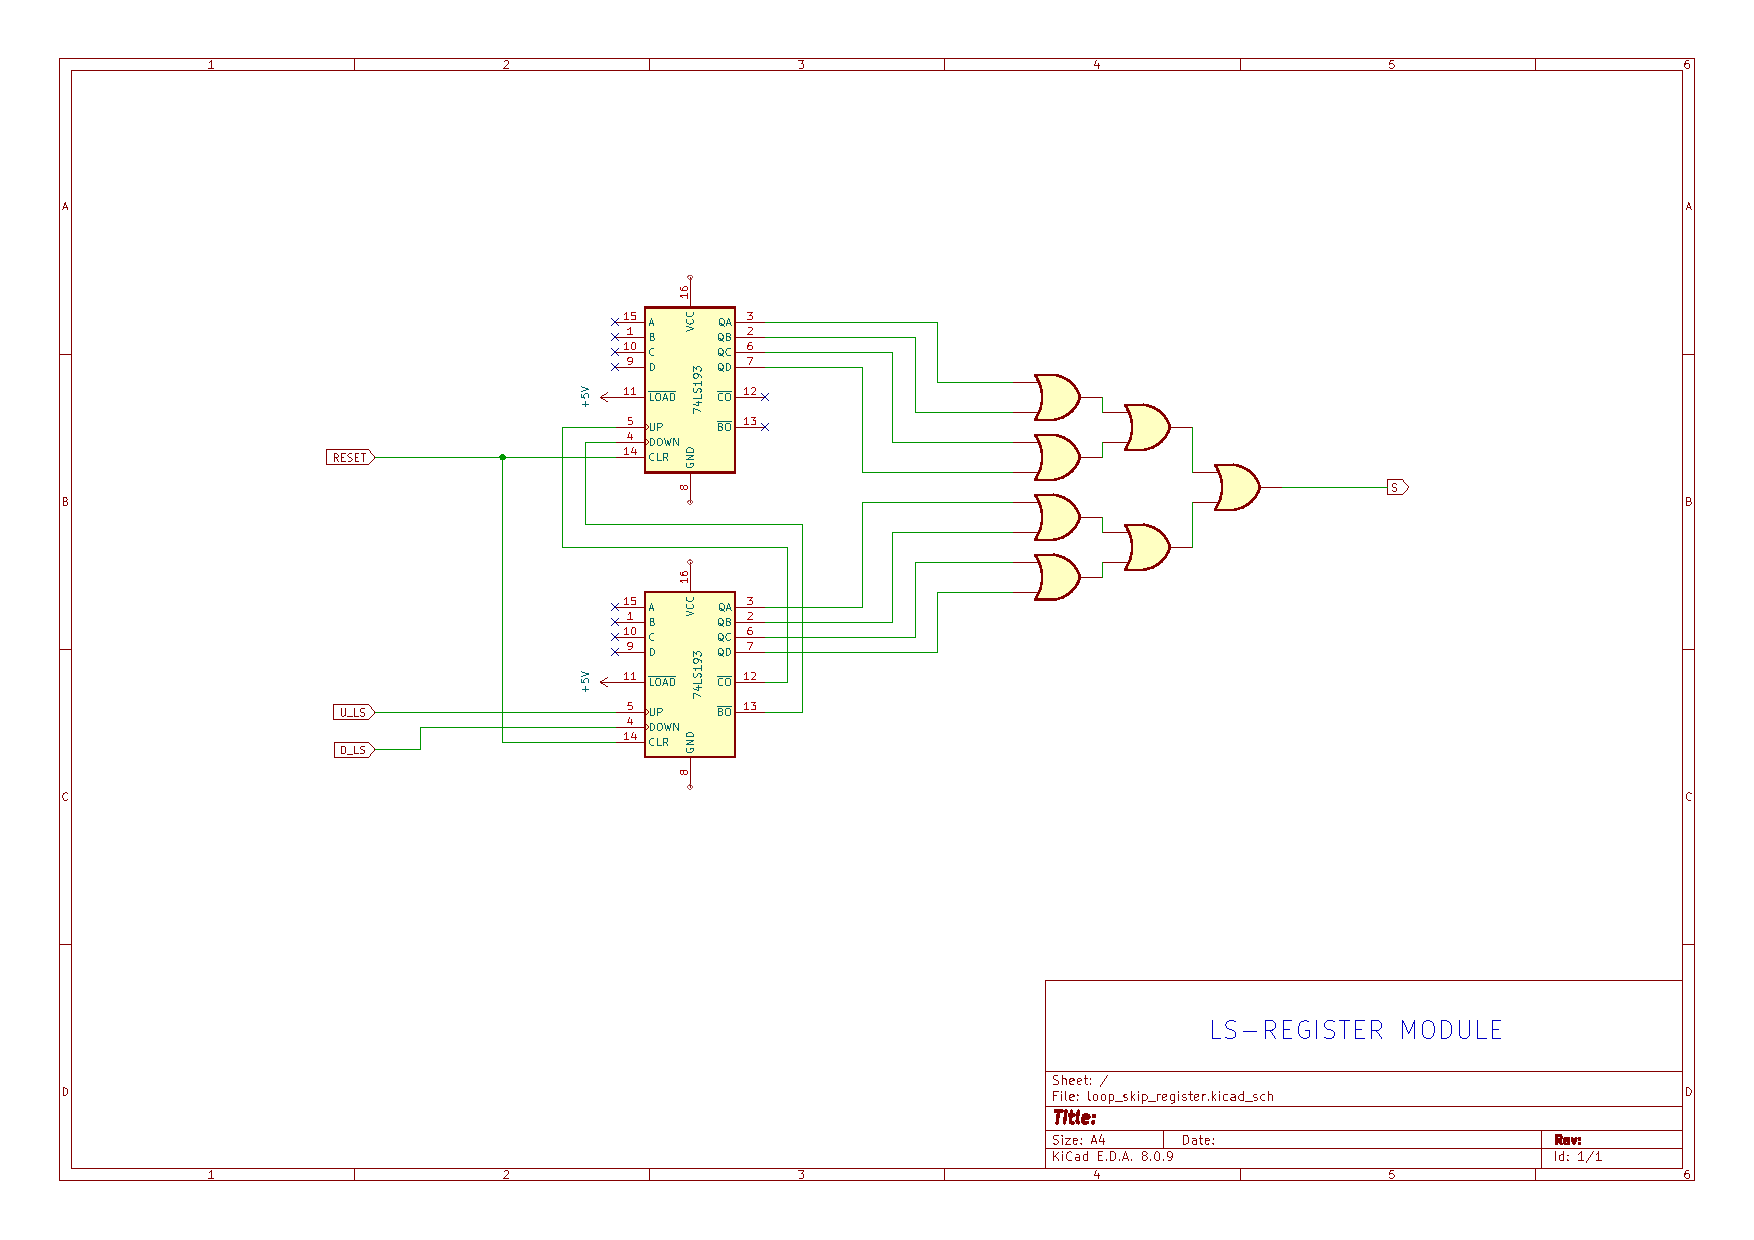
\includepdf[landscape=true]{schematics/loopskipregister.pdf}
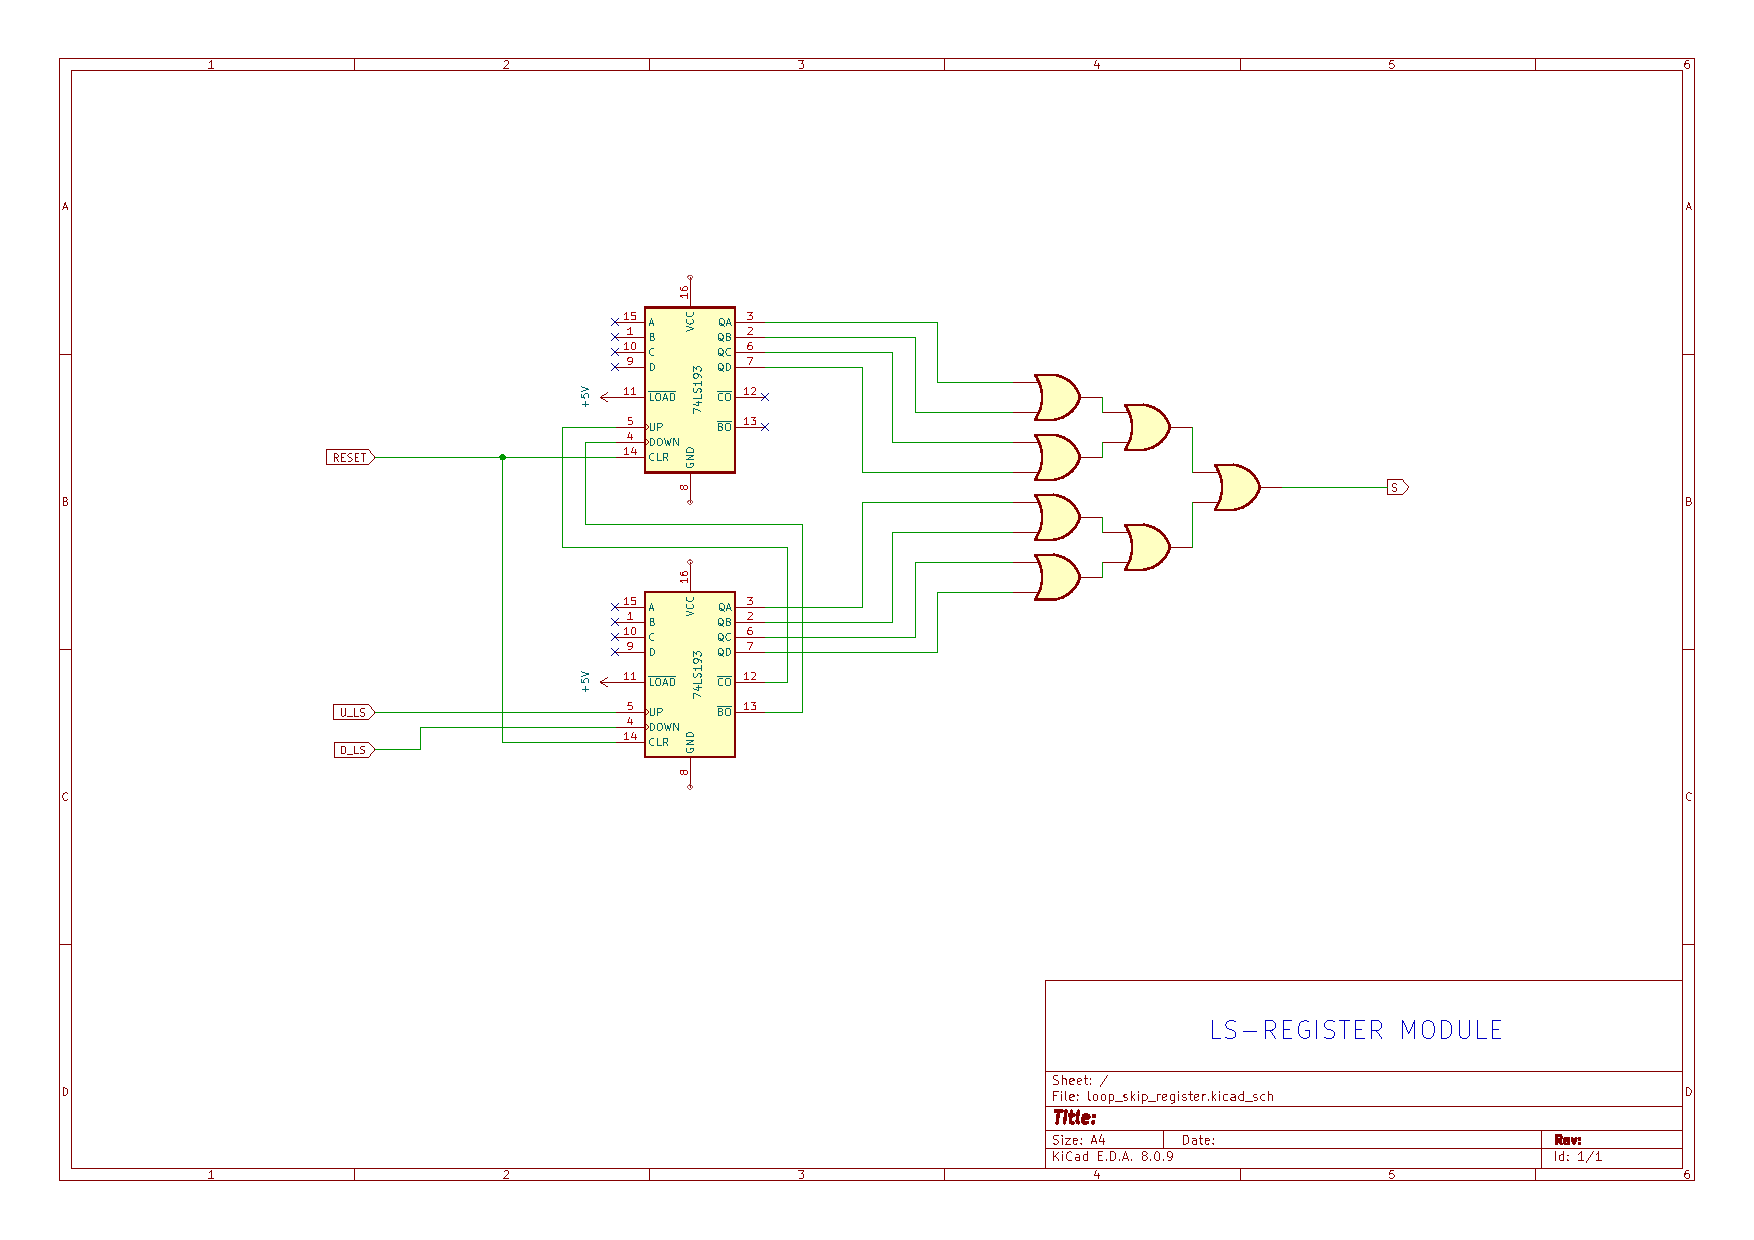
\includepdf[landscape=true]{schematics/loopskipregister.pdf}
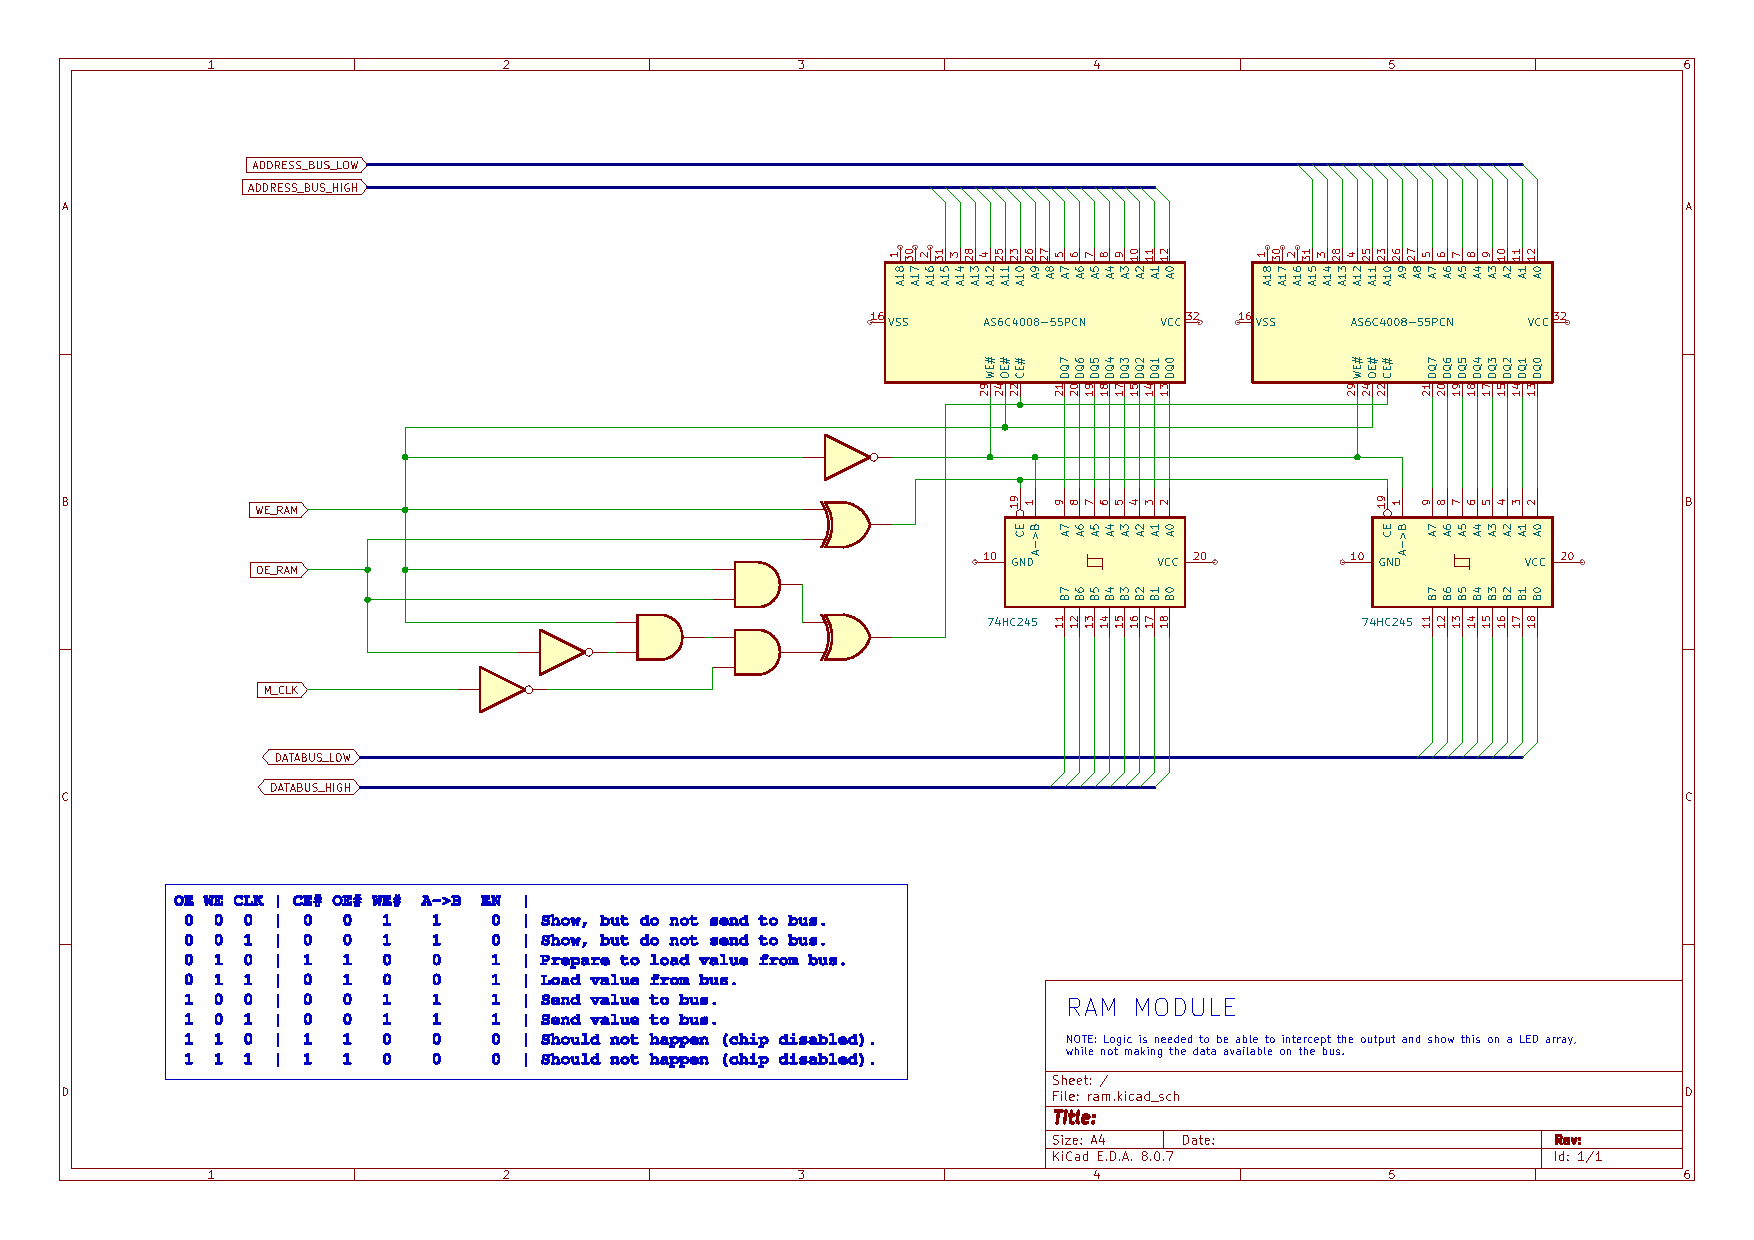
\includepdf[landscape=true]{schematics/rammodule.pdf}
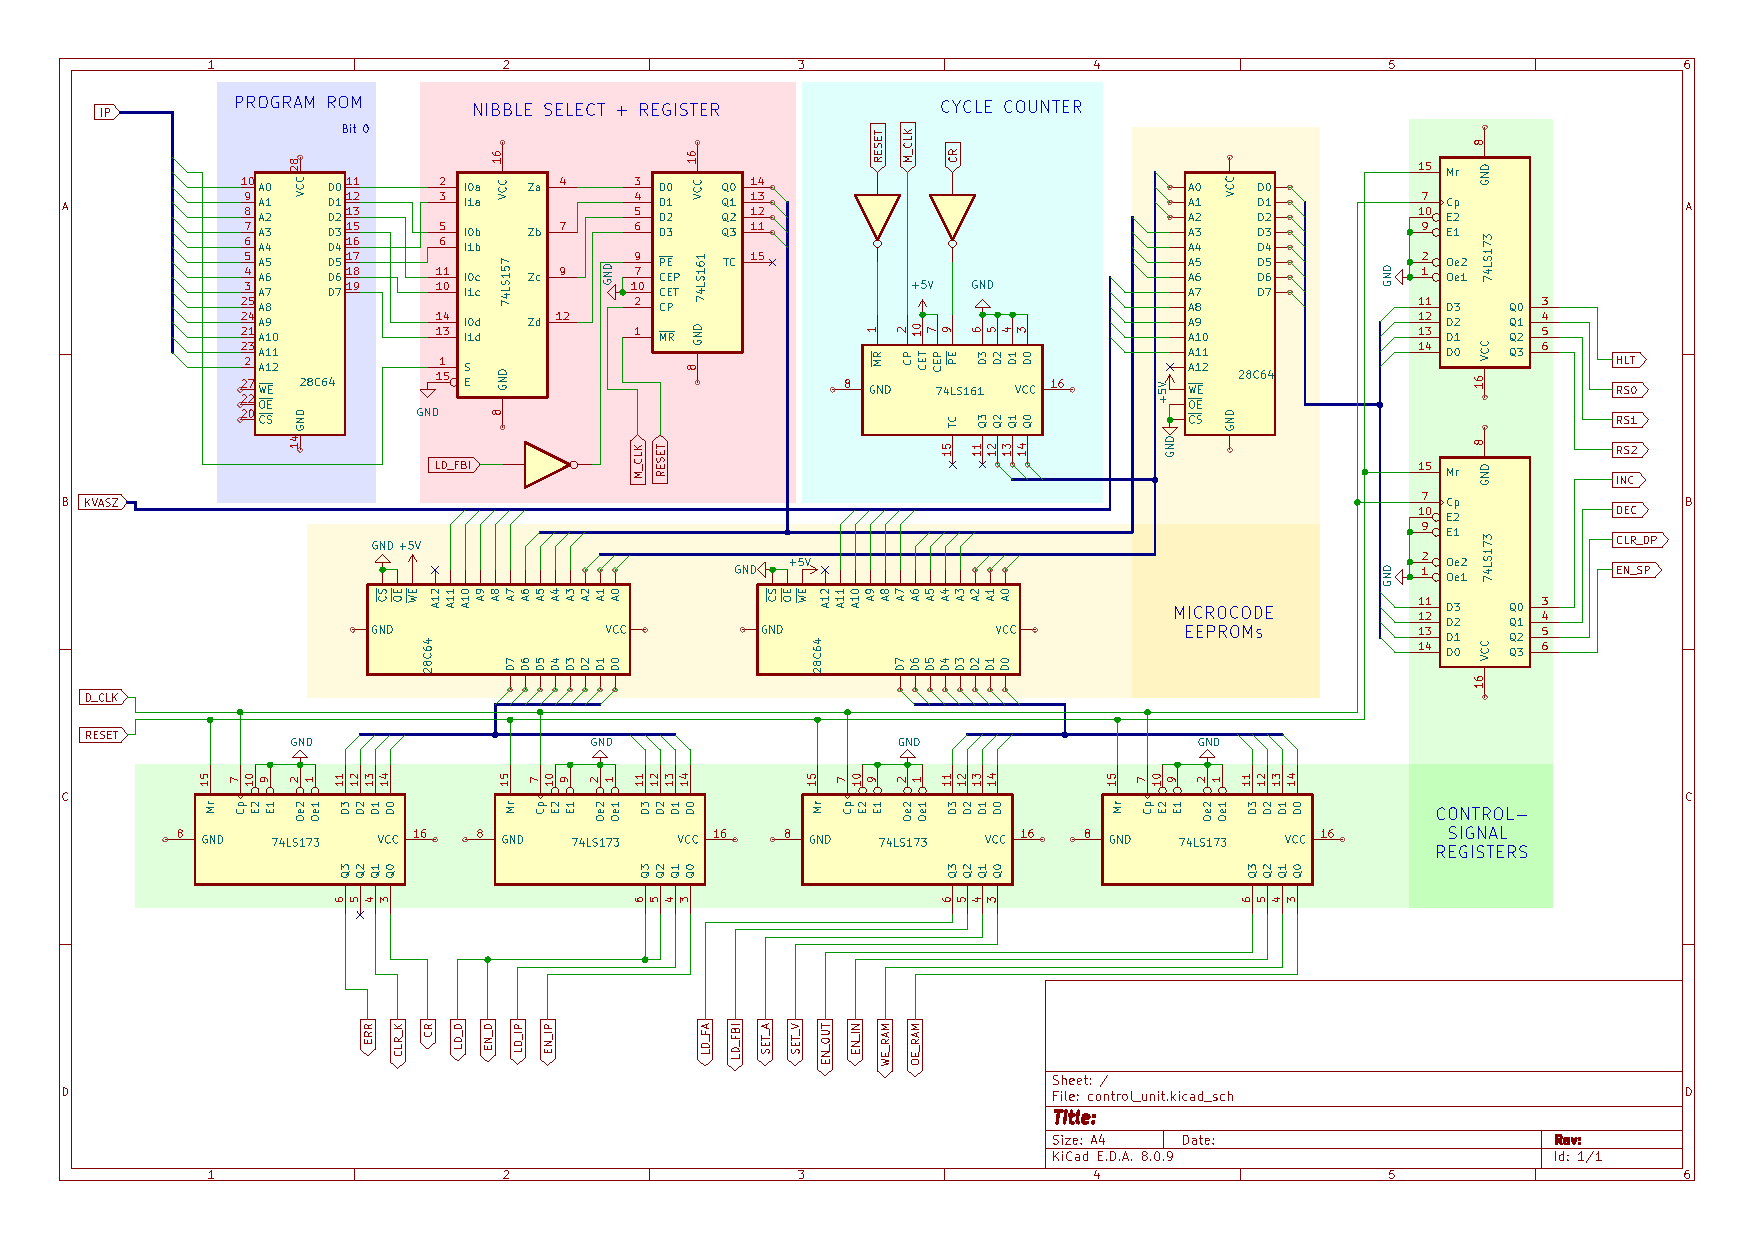
\includepdf[landscape=true]{schematics/controlunit.pdf}
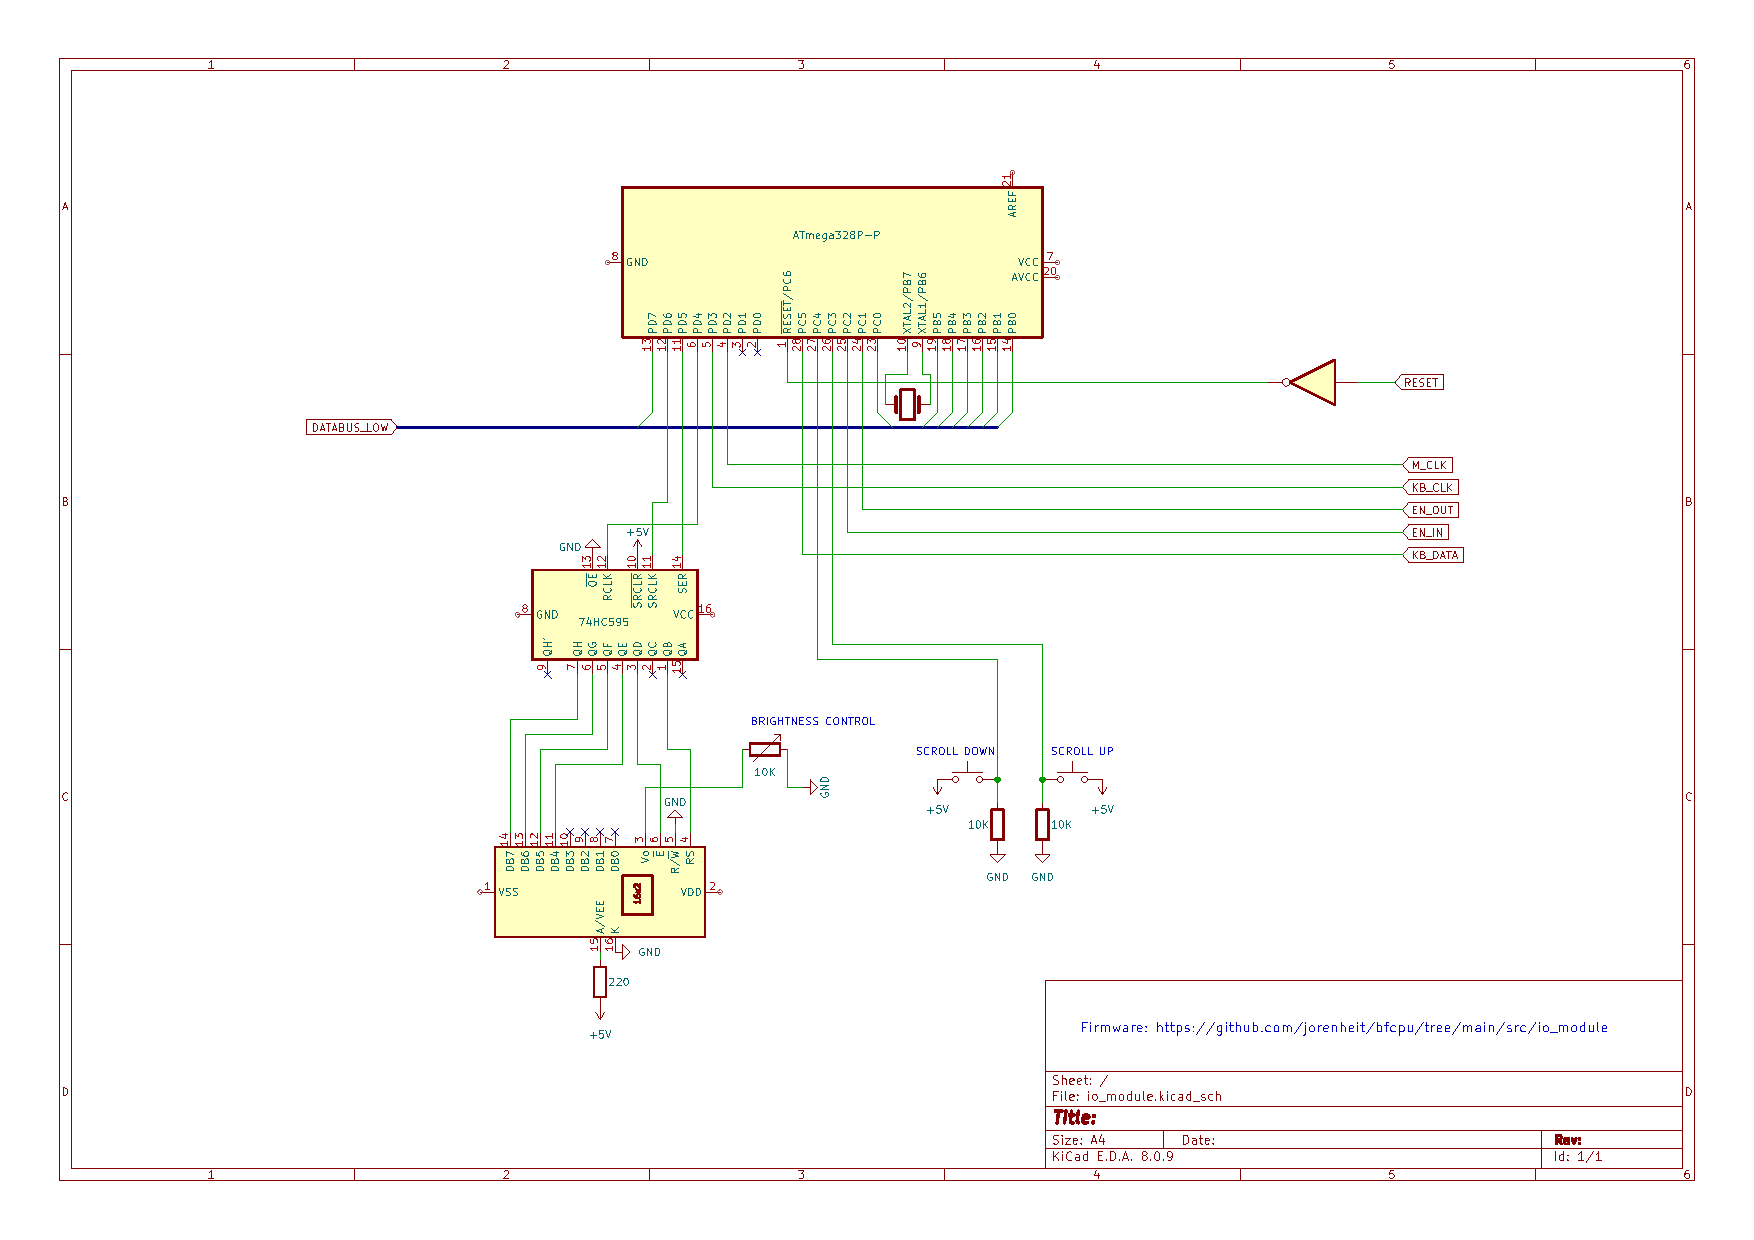
\includepdf[landscape=true]{schematics/iomodule.pdf}
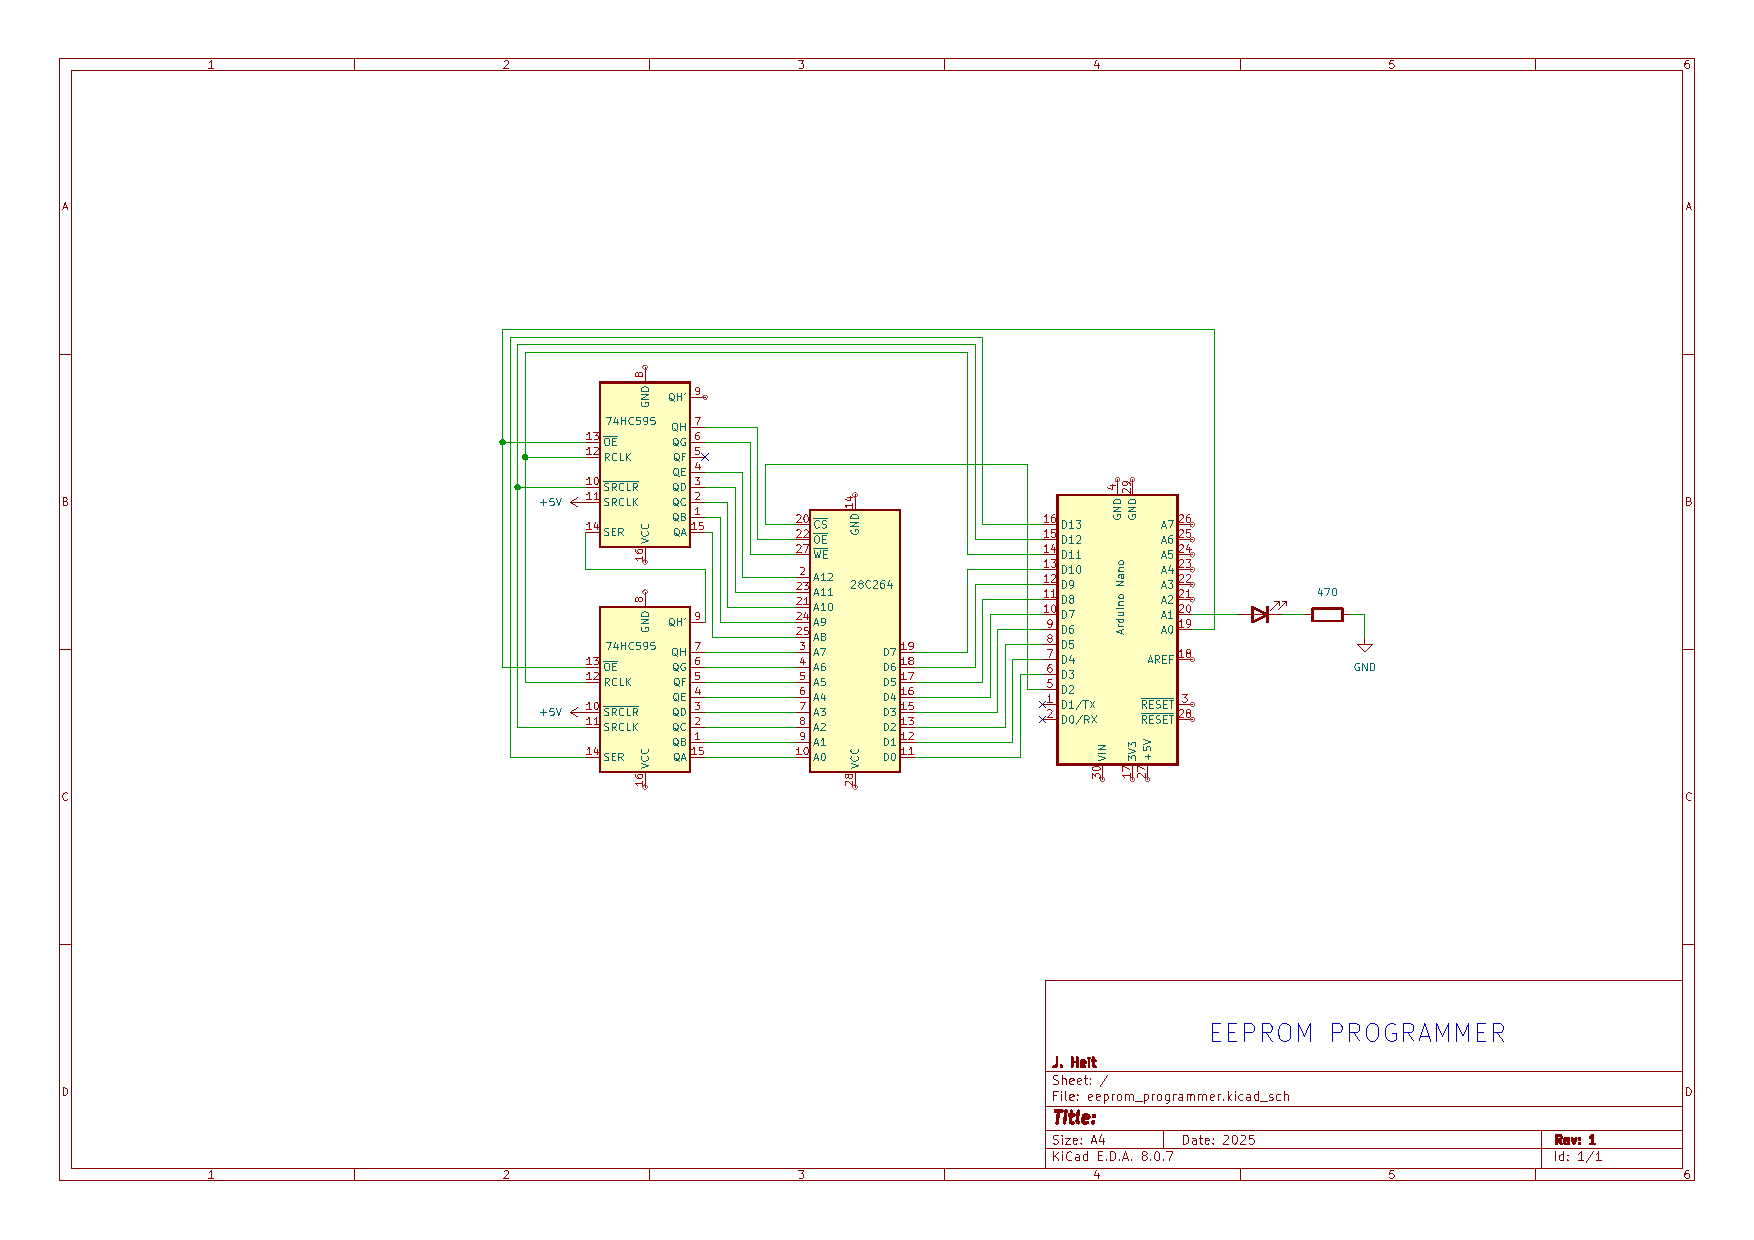
\includepdf[landscape=true]{schematics/eeprom_programmer.pdf}
